\documentclass[11pt]{beamer}

\usepackage[utf8]{inputenc}
\usepackage{hyperref}

\usetheme{Singapore}

\definecolor{DarkRed}{rgb}{0.50,0,0}
\definecolor{DarkGreen}{rgb}{0,0.50,0}
\definecolor{DarkBlue}{rgb}{0,0,0.50}
\definecolor{Black}{rgb}{0,0,0}

\newcommand{\ttdr}[1]{{\tt{\color{DarkRed} #1}}}
\newcommand{\emdr}[1]{{\em{\color{DarkRed} #1}}}
\newcommand{\ttdg}[1]{{\tt{\color{DarkGreen} #1}}}
\newcommand{\emdg}[1]{{\em{\color{DarkGreen} #1}}}
\newcommand{\ttdb}[1]{{\tt{\color{DarkBlue} #1}}}
\newcommand{\emdb}[1]{{\em{\color{DarkBlue} #1}}}

\setbeamertemplate{frametitle}{
  \begin{centering}
    {\Large \textbf{\textmd{\insertframetitle}}}
  \end{centering}
}

\setbeamertemplate{navigation symbols}{}

\setbeamertemplate{footline}{
  \begin{center}
    {\color{DarkBlue}{\large
        \insertframenumber}
      \hspace{240pt}
      
\includegraphics[height=20pt]{png/cycling.png}}
  \end{center}
}

\begin{document}

\begin{frame}
  \vspace{25pt}
  \begin{center}
    \LARGE{
      \vspace{10pt}
      {\color{DarkGreen}{
          Time Hybrids \\}}
      \vspace{10pt}
      {\color{DarkRed}{
          Lamda Days 2024 \\}}
      \vspace{10pt}
      {\color{DarkBlue}{
          Luc Duponcheel}}}
  \end{center}

\end{frame}

\begin{frame}
  \vspace{25pt}
  \begin{center}
    \LARGE{
      {\color{DarkGreen}{
            Time Hybrids \\}}
      \vspace{10pt}
      {\color{DarkRed}{
          nova science publishers \\}}
      \vspace{10pt}
      {\color{DarkBlue}{
          A New Generic Theory of Reality \\
          Fred Van Oystaeyen}}}
  \end{center}
\end{frame}

\begin{frame}[fragile]
  \frametitle{\begin{center}Generic Theory\end{center}}
  \begin{itemize}
    \item<2-> theory of theories
    \item<3-> partially unifying framework theory where theories fit into
  \end{itemize}
\end{frame}

\begin{frame}[fragile]
  \frametitle{\begin{center}Generic Theory of Reality\end{center}}
  \begin{itemize}
    \item<2-> partially unifying framework theory where theories of reality fit
      into
      \begin{itemize}
        \item<3-> relativity theory
        \item<4-> quantum theory
      \end{itemize}
    \item<5-> until now no unifying theory for them has been agreed upon
  \end{itemize}
\end{frame}

\begin{frame}[fragile]
  \frametitle{\begin{center}Specification\end{center}}
  \begin{itemize}
    \item<2-> {\em declares} features
    \item<3-> {\em defines} laws that come with those declared features
    \item<4-> also {\em defines} features in terms of declared and defined
      features
  \end{itemize}
\end{frame}

\begin{frame}[fragile]
  \frametitle{\begin{center}Implementation\end{center}}
  \begin{itemize}
    \item<2-> {\em defines} declared features of a specification
    \item<3-> provides proofs of the laws that come with those declared
      features
  \end{itemize}
\end{frame}

\begin{frame}[fragile]
  \frametitle{\begin{center}Description \\ (as a painting)\end{center}}
  \begin{itemize}
    \item<2-> below is an informal description of a pipe \\
      
\includegraphics[height=60pt]{png/pipeDescription.png}
    \item<3-> well, not really, does it?
  \end{itemize}
\end{frame}

\begin{frame}[fragile]
  \frametitle{\begin{center}Description \\ (as a computational simulation)
    \end{center}}
  \begin{itemize}
    \item<2->

      \href{https://www.ted.com/talks/stephen_wolfram_how_to_think_computationally_about_ai_the_universe_and_everything?language=en}{{\color{DarkBlue}this
            TED talk of Stephen Wolfram}} is about a, mathematically
      well-founded, description of reality that, maybe, can, somehow, be seen
      as an implementation of the specification of the generic theory of Fred
      Van Oystaeyen
  \end{itemize}
\end{frame}

\begin{frame}[fragile]
  \frametitle{\begin{center}Continuous versus Discrete\end{center}}
  \begin{itemize}
    \item<2-> relativity theory resp. quantum theory is a macro theory resp.
      micro theory, but where do micro and macro end?
    \item<3-> traditionally, mathematics is used to deal with that in a
      continous, analytic way, using shrinking limits of time intervals
    \item<4-> recently, mathematics is used to deal with that in a discrete,
      algebraic way (if only because of the observational minimal Planck time
      unit!)
  \end{itemize}
\end{frame}

\begin{frame}[fragile]
  \frametitle{\begin{center}Discrete\end{center}}
  \begin{itemize}
    \item<2-> Stephen Wolfram's mathematics uses an expanding limit of a time
      interval starting at some time moment (think of a big bang of graph
      rewriting without specific rules), recall that it is an implementation
    \item<3-> Fred Van Oystaeyen's approach also goes for a discrete, algebraic
      way but makes no concrete choices, recall that it is a specification
  \end{itemize}
\end{frame}

\begin{frame}[fragile]
  \frametitle{\begin{center}Generic Theory of Mathematics as a
      foundation\end{center}}
  \begin{itemize}
    \item<2-> Category Theory is a partially unifying framework theory where
      theories of mathematics fit into
      \begin{itemize}
        \item<3-> probability
        \item<4-> geometry (topology)
        \item<5-> others
      \end{itemize}
    \item<6-> Category theory is, just like reality, compositional
  \end{itemize}
\end{frame}

\begin{frame}[fragile]
  \frametitle{\begin{center}Virtual Topology\end{center}}
  \begin{itemize}
    \item<2-> Fred Van Oystayen's Virtual Topology is, as far as I know, the
      most abstract (read: simplest) geometry as far as being useful for
      modeling reality
    \item<3-> Virtual Topology is pointfree (cfr Category Theory)
  \end{itemize}
\end{frame}

\begin{frame}[fragile]
  \frametitle{\begin{center}Program language notation\end{center}}
  \begin{itemize}
    \item<2-> Mathematical notation can overwhelm you \\
      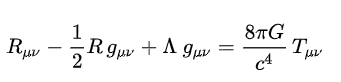
\includegraphics[height=30pt]{png/formula.png}
    \item<3-> Natural language notation can confuse you
      \begin{itemize}
        \item<4-> many words used for one concept without explanantion
        \item<5-> one word used for many concepts without defining context
      \end{itemize}
    \item<6-> Program language notation is required to be precise and,
      therefore may also overwhelm you, but the benefit is that it is checked
      by a type system that, by the way, is not overwhelmed by it
  \end{itemize}
\end{frame}

\begin{frame}[fragile]
  \frametitle{\begin{center}Category\end{center}}
  {\color{DarkGreen}
    \footnotesize{
      \footnotesize{
        \begin{verbatim}
  trait Category[BTC[_, _]]
    extends BtcComposition[BTC], BtcUnit[BTC]:
  \end{verbatim}}}}
\end{frame}

\begin{frame}[fragile]
  \frametitle{\begin{center}CategoryLaws\end{center}}
  {\color{DarkGreen}
    \footnotesize{
      \begin{verbatim}    
    trait CategoryLaws[L[_]: Law]:
  
      def leftIdentity[Z, Y]: BTC[Z, Y] => L[BTC[Z, Y]] =
        z2y => { i `o` z2y } `=` { z2y }
  
      def rightIdentity[Z, Y]: BTC[Z, Y] => L[BTC[Z, Y]] =
        z2y => { z2y `o` i } `=` { z2y }
  \end{verbatim}}}
\end{frame}

\begin{frame}[fragile]
  \frametitle{\begin{center}BtcComposition\end{center}}
  {\color{DarkGreen}
    \footnotesize{
      \begin{verbatim}
  trait BtcComposition[BTC[_, _]]:
  
    extension [Z, Y, X](y2x: BTC[Y, X])
      def `o`(z2y: BTC[Z, Y]): BTC[Z, X]
  \end{verbatim}}}
\end{frame}

\begin{frame}[fragile]
  \frametitle{\begin{center}BtcCompositionLaws\end{center}}
  {\color{DarkGreen}
    \footnotesize{
      \begin{verbatim}
  trait CompositionLaws[L[_]: Law]:

    def associativity[Z, Y, X, W]
        : BTC[X, W] => BTC[Y, X] => BTC[Z, Y] => L[BTC[Z, W]] =
      x2w => y2x => z2y =>
        { (x2w `o` y2x) `o` z2y } `=` { x2w `o` (y2x `o` z2y) }
  \end{verbatim}}}
\end{frame}

\begin{frame}[fragile]
  \frametitle{\begin{center}BtcUnit\end{center}}
  {\color{DarkGreen}
    \footnotesize{
      \begin{verbatim}
    trait BtcUnit[BTC[_, _]]:

      def i[Z]: BTC[Z, Z]
  \end{verbatim}}}
\end{frame}

\begin{frame}[fragile]
  \frametitle{\begin{center}Time\end{center}}
  {\color{DarkGreen}
    \footnotesize{
      \begin{verbatim}
    trait Time[Moment: Arbitrary: Ordered]
  \end{verbatim}}}
  \begin{itemize}
    \item<2-> this allows us to
      \begin{itemize}
        \item<3-> write statements involving arbitrary time moments
        \item<4-> state that one time moment is before another one
      \end{itemize}
  \end{itemize}
\end{frame}

\begin{frame}[fragile]
  \frametitle{\begin{center}Universe\end{center}}
  {\color{DarkGreen}
    \footnotesize{
      \begin{verbatim}
    trait Universe[
      Set[_]: Sets,
      Morphism[_, _]: Category: ActingUponFunction,
      Moment: Time,
      State: [_] =>> VirtualTopology[
        Set, 
        State
      ]: [_] =>> Functor[
        [_, _] =>> MomentMorphism,
        Morphism,
        [_] =>> State
      ]
    ]
  \end{verbatim}}}
\end{frame}

\begin{frame}[fragile]
  \frametitle{\begin{center}Universe continued\end{center}}
  \begin{itemize}
    \item<2-> this allows us to
      \begin{itemize}
        \item<3-> write statements using topological features of universe
          states
        \item<4-> write statements relating time moment transitions, to
          universe state morphisms (think of an dynamic, expanding universe)
      \end{itemize}
  \end{itemize}
\end{frame}

\begin{frame}[fragile]
  \frametitle{\begin{center}An example: immobility\end{center}}
  \begin{itemize}
    \item<2-> immobility can be expressed without mentioning real numbers for
      time and space
    \item<3-> some history of geometry
      \begin{itemize}
        \item<4-> Euclides did not use numbers to measure with
        \item<5-> Pythagoras showed that rational numbers were not enough
      \end{itemize}
  \end{itemize}
\end{frame}

\begin{frame}[fragile]
  \frametitle{\begin{center}immobileAfter\end{center}}
  {\color{DarkGreen}
    \footnotesize{
      \begin{verbatim}
    val immobileAfter
      : MomentMorphism => L[Function[PreThingsSet, State]] =
    mm =>
      {
        pts2s `o` mm2ptsf(mm)
      } `=` {
        mm2sm(mm) `a` pts2s
      }
  \end{verbatim}}}
\end{frame}

\begin{frame}[fragile]
  \frametitle{\begin{center}immobileAfter\end{center}}
  {\color{DarkGreen}
    \footnotesize{
      \begin{verbatim}
    val immobileOnInterval
      : MomentMorphism => PreThingsSet => L[State] =
      case (bm, em) =>
        val mi: Interval[Moment] = interval apply ((bm, em))
        pts =>
          all apply {
            for {
              m <- mi
            } yield {
              {
                (pts2s `o` mm2ptsf((bm, m)))(pts)
              } `=` {
                (mm2sm((bm, m)) `a` pts2s)(pts)
              }
            }
          }
  \end{verbatim}}}
\end{frame}

\begin{frame}[fragile]
  \frametitle{\begin{center}Reality goes beyond Imagination\end{center}}
  \begin{itemize}
    \item<2-> the \ttdg{`a`} in the formula is not morphism composition
      \ttdg{`o`}
    \item<3-> the \ttdg{`a`} in the formula is an action of morphism
      \ttdg{mm2sm(mm)} on the place function \ttdg{pts2s}
    \item<4-> cfr a monoid acting upon a set
    \item<4-> cfr rotations acting upon a Rubic Cube
  \end{itemize}
\end{frame}

\begin{frame}[fragile]
  \frametitle{\begin{center}More Information\end{center}}
  \ttdg{https://github.com/LucDuponcheelAtGitHub/timeHybrids}
\end{frame}

\begin{frame}[fragile]
  \frametitle{\begin{center}THANKS FOR ATTENDING\end{center}}
  \begin{center}
    
\includegraphics[height=190pt]{png/cycling.png}
  \end{center}
\end{frame}

\end{document}
